\section{Introduction to Machine Learning}

\begin{frame}{Learning Goals}
\begin{itemize}
  \item Define machine learning as a prediction problem with inputs, outputs, data, and an evaluation objective.
  \pause
  \item Distinguish rule-based decision logic from machine learning and identify common machine learning task types.
  \pause
  \item Explain datasets, features, labels, and train, validation, and test splits.
  \pause
  \item Explain k-nearest neighbors (k-NN) as a non-parametric method for classification, regression, retrieval, and anomaly scoring.
  \pause
  \item Compute simple distance measures, explain formal generalization, and analyze how the choice of $k$ affects accuracy and cost.
\end{itemize}
\end{frame}

\begin{frame}{Reading Resources}
\begin{itemize}
  \item We do not follow a single textbook strictly.
  \pause
  \item Core theory reference: \textit{Foundations of Machine Learning} (Mohri et al.).
  \pause
  \item Statistical learning reference: \textit{The Elements of Statistical Learning} (Hastie, Tibshirani, Friedman).
  \pause
  \item Probabilistic modeling reference: \textit{Pattern Recognition and Machine Learning} (Bishop).
  \pause
  \item Broad machine learning reference: \textit{Machine Learning: A Probabilistic Perspective} (Murphy).
  \pause
  \item Deep learning reference: \textit{Deep Learning} (Goodfellow, Bengio, Courville).
  \pause
  \item Practical references: scikit-learn docs (\url{https://scikit-learn.org/stable/}) and PyTorch docs (\url{https://pytorch.org/docs/stable/}).
  \pause
  \item We also use selected papers, lecture notes, benchmark datasets, and practical case studies.
\end{itemize}
\end{frame}

\begin{frame}{Advanced AI Covers Different Kinds of Topics}
\begin{itemize}
  \item Some topics are \textbf{classic foundations}: regression, classification, nearest neighbors, generalization, kernels, clustering.
  \pause
  \item Some topics are \textbf{specialized methods}: probabilistic models, structured prediction, search, graphical models, sequence models.
  \pause
  \item Some topics are \textbf{harder modern systems}: deep learning, representation learning, large-scale retrieval, generative models, reinforcement learning.
  \pause
  \item The course therefore cannot be organized as ``finish one book from page 1 to the end''.
  \pause
  \item Instead, we build a route from core ideas to harder models, using multiple references when needed.
\end{itemize}
\end{frame}

\begin{frame}{How We Navigate This Course}
\begin{columns}[T]
\column{0.48\textwidth}
\textbf{What we prioritize first}
\begin{itemize}
  \item concepts that define a learning problem
  \pause
  \item algorithms with clear geometric or statistical intuition
  \pause
  \item methods that can be implemented from scratch
  \pause
  \item examples that connect theory to real applications
\end{itemize}

\pause
\column{0.48\textwidth}
\textbf{How books are used}
\begin{itemize}
  \item Mohri et al.: learning theory and formal guarantees
  \pause
  \item Bishop: modeling intuition and probabilistic methods
  \pause
  \item scikit-learn docs: practical usage and standard workflows
  \pause
  \item selected papers: newer methods beyond the books
\end{itemize}
\end{columns}

\vspace{0.5em}
\pause
\begin{block}{Course principle}
We start from methods that are simple enough to analyze carefully, then revisit the same questions for stronger and more complex models.
\end{block}
\end{frame}

\begin{frame}{What Is Machine Learning?}
\begin{rldefinition}
Machine learning studies algorithms that learn patterns from data and improve
prediction performance on unseen examples.
\end{rldefinition}

\vspace{0.5em}
Formal setup:
\begin{itemize}
  \item Input space: $X$
  \pause
  \item Output space: $Y$
  \pause
  \item Hypothesis: $h: X \to Y$
  \pause
  \item Goal: optimize an objective (for example, minimize loss or maximize reward)
\end{itemize}
\end{frame}

\begin{frame}{Rule-based Logic vs Machine Learning (Manufacturing Robotics)}
\begin{columns}[T]
\column{0.48\textwidth}
\textbf{Rule-based manufacturing}
\begin{itemize}
  \item Engineer writes fixed decision rules and motion sequence
  \pause
  \item Example: identical parts arrive in the same pose on a conveyor
  \pause
  \item Robot picks, places, and routes using sensor thresholds and pre-defined coordinates
  \pause
  \item Strong when the environment is stable and variation is small
\end{itemize}

\pause
\column{0.48\textwidth}
\textbf{Machine learning manufacturing}
\begin{itemize}
  \item Model learns decision boundaries from labeled examples
  \pause
  \item Example: parts arrive with different poses, shapes, or visible defects
  \pause
  \item Robot uses images or sensor features to classify, reject, or sort parts
  \pause
  \item Strong when perception is difficult but the task objective is clear
\end{itemize}
\end{columns}

\pause
\begin{rlintuition}
Use rule-based control when the factory cell is highly structured. Use machine learning when the main difficulty is recognizing patterns under variation.
\end{rlintuition}
\end{frame}

\begin{frame}{Manufacturing Example: Rule-based vs Machine Learning}
\centering
\includegraphics[width=0.94\textwidth]{figures/intro/manufacturing_rule_vs_ml.pdf}

\vspace{0.4em}
\begin{itemize}
  \item Left: fixed parts and fixed routing logic.
  \pause
  \item Right: visual variation requires learned recognition before action.
\end{itemize}
\end{frame}

\begin{frame}{Why Machine Learning in Practice?}
\begin{itemize}
  \item Hard to write explicit rules for many tasks.
  \pause
  \item Data can reveal patterns that manual rules miss.
  \pause
  \item Performance can improve as more data becomes available.
\end{itemize}

\pause
\begin{rlintuition}
Use machine learning when pattern complexity is high and reliable labeled
or unlabeled data is available.
\end{rlintuition}
\end{frame}

\begin{frame}{Real-World Examples}
\begin{columns}[T]
\column{0.48\textwidth}
\textbf{Consumer products}
\begin{itemize}
  \item Spam and phishing detection
  \pause
  \item Search and recommendation
  \pause
  \item Voice assistants
\end{itemize}

\pause
\textbf{Finance}
\begin{itemize}
  \item Fraud detection
  \pause
  \item Credit risk estimation
\end{itemize}

\pause
\column{0.48\textwidth}
\textbf{Healthcare}
\begin{itemize}
  \item Imaging triage
  \pause
  \item Readmission risk prediction
\end{itemize}

\pause
\textbf{Industry}
\begin{itemize}
  \item Predictive maintenance
  \pause
  \item Demand forecasting
\end{itemize}
\end{columns}
\end{frame}

\begin{frame}{Standard Task Types}
\begin{itemize}
  \item Classification: predict categories.
  \pause
  \item Regression: predict continuous values.
  \pause
  \item Ranking: order items by relevance.
  \pause
  \item Clustering: group unlabeled data.
  \pause
  \item Dimensionality reduction: compress representation.
  \pause
  \item Generative modeling: synthesize text, images, code, audio.
\end{itemize}
\end{frame}

\begin{frame}{Simple Task-Type to Algorithm Map}
\begin{itemize}
  \item Classification: logistic regression, decision trees, k-nearest neighbors (k-NN)
  \pause
  \item Regression: linear/ridge regression, regression trees
  \pause
  \item Clustering: k-means, hierarchical clustering
  \pause
  \item Dimensionality reduction: principal component analysis (PCA), kernel PCA
  \pause
  \item Ranking: pairwise linear ranking models
\end{itemize}
\end{frame}

\begin{frame}{Running Example: Spam Detection}
\begin{itemize}
  \item Input: email features (keywords, sender patterns, metadata).
  \pause
  \item Output: label in $\{\text{spam}, \text{non-spam}\}$.
  \pause
  \item Model: classifier selected from a hypothesis set.
\end{itemize}

\pause
\begin{rlquestion}
Which features would you trust most for modern spam detection?
\end{rlquestion}
\end{frame}

\begin{frame}{Graphic: Learning Pipeline}
\centering
\begin{tikzpicture}[
  node distance=0.9cm and 0.45cm,
  box/.style={draw=RLBlue, rounded corners, thick, minimum height=1.1cm, minimum width=2.1cm, align=center, fill=RLGray},
  arr/.style={->, thick, color=RLBlue}
]
\node[box] (data) {Raw\\Data};
\node[box, right=of data] (features) {Feature/\\Representation};
\node[box, right=of features] (train) {Train\\Model};
\node[box, right=of train] (val) {Validate\\Tune};
\node[box, right=of val] (test) {Test\\Report};

\draw[arr] (data) -- (features);
\draw[arr] (features) -- (train);
\draw[arr] (train) -- (val);
\draw[arr] (val) -- (test);
\end{tikzpicture}

\vspace{0.6em}
\pause
\footnotesize This separation is a minimum standard\\
\footnotesize for trustworthy ML results.
\end{frame}

\begin{frame}{Core Terminology and Examples}
\small
\begin{columns}[T]
\column{0.48\textwidth}
\begin{itemize}
  \item Dataset: $S=\{(x_i,y_i)\}_{i=1}^m$
  \pause
  \item Feature vector: $x_i \in \mathbb{R}^d$
  \pause
  \item Examples: email word counts, robot sensor values
  \pause
  \item Label: $y_i$ (class or real value)
  \pause
  \item Predictor: $\hat{y}=f_\theta(x)$
  \pause
  \item Example models: linear/logistic regression, trees, k-nearest neighbors (k-NN), neural nets
\end{itemize}

\pause
\column{0.48\textwidth}
\begin{itemize}
  \item Hypothesis class $\mathcal{H}$: candidate predictors
  \pause
  \item Loss: $\ell(y,\hat{y})$ (one common objective)
  \pause
  \item Empirical risk minimization (ERM) objective (many models):\\
  $J(\theta)=\frac{1}{m}\sum_{i=1}^m \ell(y_i,f_\theta(x_i))+\lambda\Omega(\theta)$
  \pause
  \item Other goals: maximize likelihood (Naive Bayes, Gaussian mixture model, GMM), maximize information gain (trees), neighbor voting (k-nearest neighbors, k-NN)
  \pause
  \item Hyperparameters: $\lambda$, learning rate, model size
\end{itemize}
\end{columns}
\end{frame}

\begin{frame}{Problem-Solving Stages (Model-Agnostic)}
\begin{enumerate}
  \item Define task, output type, and metric.
  \pause
  \item Prepare data and representation (features or embeddings).
  \pause
  \item Choose method family:
  \begin{itemize}
    \item parametric (for example linear models, neural nets),
    \item non-parametric/structural (for example k-nearest neighbors, k-NN; trees; principal component analysis, PCA; kernels).
  \end{itemize}
  \pause
  \item Fit or construct method:
  \begin{itemize}
    \item train parameters, or
    \item build structure/decomposition.
  \end{itemize}
  \pause
  \item Validate using held-out data or internal criteria (for unsupervised tasks).
  \pause
  \item Test, interpret, and monitor after deployment.
\end{enumerate}
\end{frame}

\begin{frame}{Train, Validation, Test Split}
\begin{columns}[T]
\column{0.48\textwidth}
\textbf{Training set}
\begin{itemize}
  \item Fit model parameters
  \pause
  \item Largest portion of data
\end{itemize}

\pause
\column{0.48\textwidth}
\textbf{Validation set}
\begin{itemize}
  \item Model selection
  \pause
  \item Hyperparameter tuning
\end{itemize}
\end{columns}

\vspace{0.5em}
\pause
\textbf{Test set}
\begin{itemize}
  \item Final unbiased performance estimate
\end{itemize}

\pause
\begin{rlpitfall}
Keep the test set untouched until final evaluation.
\end{rlpitfall}
\end{frame}

\begin{frame}{Non-Parametric Baseline: k-Nearest Neighbors (k-NN)}
\begin{columns}[T]
\column{0.5\textwidth}
\textbf{Algorithm}
\begin{enumerate}
  \item Store labeled training samples.
  \pause
  \item Choose distance metric and $k$.
  \pause
  \item Find nearest $k$ neighbors for query $x_q$.
  \pause
  \item Predict by vote/average.
\end{enumerate}

\pause
\column{0.48\textwidth}
\textbf{Quick sample (classification)}
\begin{itemize}
  \item Query: new email $x_q$
  \pause
  \item $k=5$ nearest labels:
  \[
  [\text{spam},\text{spam},\text{non},\text{spam},\text{non}]
  \]
  \pause
  \item Majority vote $\Rightarrow \hat{y}=\text{spam}$
\end{itemize}
\end{columns}
\end{frame}

\begin{frame}{k-Nearest Neighbors (k-NN) Classification: Effect of k}
\centering
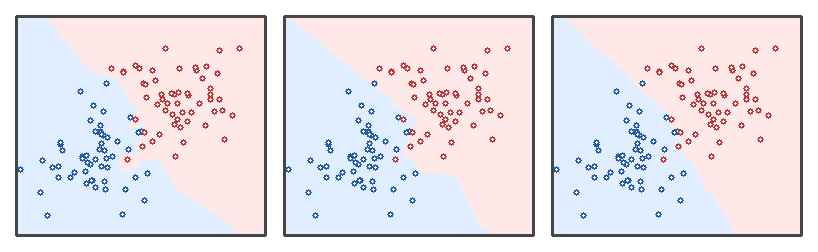
\includegraphics[width=0.96\textwidth]{figures/knn/knn_classification_k_effect.pdf}

\vspace{0.4em}
\footnotesize Left to right: $k=1$, $k=5$, $k=15$.  
\footnotesize Small $k$ is flexible/noisy; larger $k$ is smoother.
\end{frame}

\begin{frame}{k-Nearest Neighbors (k-NN) Regression: Effect of k}
\centering
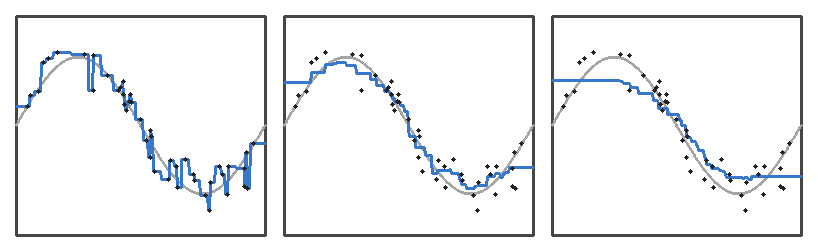
\includegraphics[width=0.96\textwidth]{figures/knn/knn_regression_k_effect.pdf}

\vspace{0.4em}
\footnotesize Left to right: $k=1$, $k=5$, $k=15$.  
\footnotesize Prediction becomes smoother as $k$ increases.
\end{frame}

\begin{frame}{k-Nearest Neighbors (k-NN) Practical Setup and Scaling}
\centering
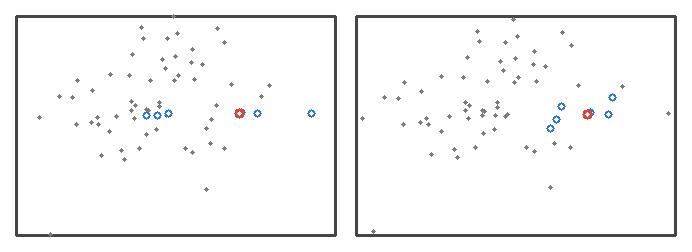
\includegraphics[width=0.76\textwidth]{figures/knn/knn_scaling_effect.pdf}

\vspace{0.2em}
\pause
\begin{itemize}
  \item Left: neighbors without scaling. Right: neighbors after standardization.
  \pause
  \item Select $k$ by validation (small $k$: high variance, large $k$: high bias).
  \pause
  \item Optional weighted voting: closer neighbors get larger weight.
  \pause
  \item Strengths: simple, strong baseline, no heavy training.
  \pause
  \item Limitations: slow inference for large datasets, sensitive to irrelevant features.
\end{itemize}
\end{frame}

\begin{frame}{Distance Metrics Change the Neighborhood}
\small
\begin{itemize}
  \item The distance function defines which samples become nearest neighbors.
\end{itemize}
\pause
For two-feature vectors $x=(x_1,x_2)$ and $z=(z_1,z_2)$:
\[
d_{L_2}(x,z)=\sqrt{(x_1-z_1)^2+(x_2-z_2)^2}
\]
\pause
\[
d_{L_1}(x,z)=|x_1-z_1|+|x_2-z_2|
\]
\pause
\[
s_{\cos}(x,z)=\frac{x_1z_1+x_2z_2}{\sqrt{x_1^2+x_2^2}\sqrt{z_1^2+z_2^2}},
\qquad
d_{\cos}(x,z)=1-s_{\cos}(x,z)
\]
\pause
\begin{itemize}
  \item Euclidean ($L_2$ norm): common for continuous features.
  \pause
  \item Manhattan ($L_1$ norm): can be more robust to outliers.
  \pause
  \item Cosine: compares direction, common with embeddings.
\end{itemize}
\end{frame}

\begin{frame}{Two-Feature Distance Example}
\small
Query $q=(2,5)$, candidate $A=(3,3)$, candidate $B=(5,4)$.
\pause
\begin{itemize}
  \item Euclidean:
  \[
  d_{L_2}(q,A)=\sqrt{(2-3)^2+(5-3)^2}=\sqrt{5}\approx2.24,\;
  d_{L_2}(q,B)=\sqrt{10}\approx3.16
  \]
  \pause
  \item Manhattan:
  \[
  d_{L_1}(q,A)=|2-3|+|5-3|=3,\;
  d_{L_1}(q,B)=|2-5|+|5-4|=4
  \]
  \pause
  \item Cosine similarity:
  \[
  s_{\cos}(q,A)\approx0.92,\qquad s_{\cos}(q,B)\approx0.87
  \]
\end{itemize}

\pause
\begin{rlintuition}
For this 2-feature example, all three metrics select $A$ as closer than $B$.
\end{rlintuition}
\end{frame}

\begin{frame}{k-Nearest Neighbors (k-NN) Computational Cost and Indexing}
\small
\textbf{Worked example}
\begin{itemize}
  \item Assume $n=200{,}000$ vectors, $d=64$, and $5{,}000$ queries.
  \pause
  \item Brute-force per query: $n\cdot d=12.8$ million feature comparisons.
  \pause
  \item Total for 5,000 queries: $\approx 64$ billion feature comparisons.
  \pause
  \item Vector memory (float32): $n\cdot d\cdot 4 \approx 51.2$ megabytes (MB), without index overhead.
\end{itemize}

\pause
\textbf{Acceleration example}
\begin{itemize}
  \item Approximate nearest neighbor (ANN) search with candidate list \(\approx 200\): \(200\cdot 64=12{,}800\) comparisons/query.
  \pause
  \item This is roughly three orders of magnitude fewer comparisons than brute force.
\end{itemize}
\end{frame}

\begin{frame}{Graphic: Query Cost Growth by Search Method}
\centering
\includegraphics[width=0.88\textwidth]{figures/knn/knn_indexing_tradeoff.pdf}

\vspace{0.35em}
\pause
\footnotesize Trend is illustrative: brute-force grows with \(n\), indexed/approximate nearest neighbor (ANN) methods grow much slower.
\end{frame}

\begin{frame}{k-Nearest Neighbors (k-NN) Beyond Classification and Regression}
\begin{itemize}
  \item \textbf{Anomaly detection}: score a point by distance to its nearest normal neighbors.
  \pause
  \item \textbf{Recommendation retrieval}: find users/items with similar interaction vectors.
  \pause
  \item \textbf{Missing-value imputation}: fill a missing value using neighbor average or vote.
  \pause
  \item \textbf{Near-duplicate detection}: detect highly similar documents/images.
\end{itemize}

\pause
\begin{rlintuition}
General pattern: define a distance, find neighbors, then aggregate their information.
\end{rlintuition}
\end{frame}

\begin{frame}{Case Study 1: Recommender Candidate Retrieval}
\textbf{Goal}
\begin{itemize}
  \item For each user, retrieve a small candidate set from millions of items.
\end{itemize}

\pause
\textbf{k-nearest neighbors (k-NN) formulation}
\begin{itemize}
  \item Learn user/item embeddings.
  \pause
  \item Retrieve top-$k$ nearest items by cosine similarity.
  \pause
  \item Pass candidates to a heavier ranking model.
\end{itemize}

\pause
\textbf{Why this matters}
\begin{itemize}
  \item k-NN retrieval controls recall and latency in production.
\end{itemize}
\end{frame}

\begin{frame}{Case Study 2: Industrial Anomaly Screening}
\textbf{Goal}
\begin{itemize}
  \item Detect unusual sensor patterns on machines.
\end{itemize}

\pause
\textbf{k-nearest neighbors (k-NN) idea}
\begin{itemize}
  \item Use distance to nearest healthy neighbors as anomaly score.
  \pause
  \item Large distance $\Rightarrow$ likely abnormal behavior.
\end{itemize}

\pause
\textbf{Operational notes}
\begin{itemize}
  \item Need robust scaling, drift monitoring, and periodic index refresh.
\end{itemize}
\end{frame}

\begin{frame}{Formal Definition of Generalization}
\small
Let training sample $S=\{(x_i,y_i)\}_{i=1}^m$ be drawn i.i.d. from distribution $\mathcal{D}$, and let $h_S$ be the learned predictor.
\pause
\[
R(h_S)=\mathbb{E}_{(x,y)\sim\mathcal{D}}[\ell(h_S(x),y)]
\]
\pause
\[
\hat{R}_S(h_S)=\frac{1}{m}\sum_{i=1}^{m}\ell(h_S(x_i),y_i)
\]
\pause
\[
\text{GenGap}(h_S)=R(h_S)-\hat{R}_S(h_S)
\]
\pause
\begin{itemize}
  \item Good generalization means low true risk \(R(h_S)\) and a small generalization gap.
  \pause
  \item In practice, we estimate \(R(h_S)\) using validation/test data.
\end{itemize}
\end{frame}

\begin{frame}{Generalization Through k-Nearest Neighbors (k-NN)}
\begin{itemize}
  \item Very small $k$: low bias, high variance (sensitive to noise).
  \pause
  \item Very large $k$: high bias, low variance (too smooth).
  \pause
  \item Validation data provides a practical estimate for unseen-data behavior.
  \pause
  \item Classical consistency intuition:
  \[
  k \to \infty,\qquad \frac{k}{m}\to 0
  \]
  balances locality and stability as sample size \(m\) grows.
\end{itemize}
\end{frame}

\begin{frame}{k-NN Calculation Example: Estimated Generalization Gap}
\small
Use 0--1 loss: \(\ell(\hat{y},y)=\mathbf{1}[\hat{y}\neq y]\). Suppose:
\[
m=120,\qquad n_{val}=40
\]
\pause
\begin{itemize}
  \item For \(k=1\): train errors \(=0\), validation errors \(=10\)
  \[
  \hat{R}_{train}=0/120=0,\qquad \hat{R}_{val}=10/40=0.25
  \]
  \pause
  \item For \(k=9\): train errors \(=8\), validation errors \(=6\)
  \[
  \hat{R}_{train}=8/120\approx0.067,\qquad \hat{R}_{val}=6/40=0.15
  \]
\end{itemize}

\pause
\begin{rlintuition}
Estimated gap (validation minus training) is smaller for \(k=9\), and validation error is also lower, so \(k=9\) is a better operating point here.
\end{rlintuition}
\end{frame}

\begin{frame}{Underfitting and Overfitting Through k}
\begin{itemize}
  \item Underfitting example: $k=51$ in a two-cluster problem smooths away boundaries.
  \pause
  \item Overfitting example: $k=1$ memorizes noisy labels near outliers.
  \pause
  \item Best $k$ depends on noise level, sample size, and representation quality.
\end{itemize}

\pause
\begin{rlpitfall}
Do not transfer ``good k'' from one dataset to another without re-validation.
\end{rlpitfall}
\end{frame}

\begin{frame}{Practical k-Nearest Neighbors (k-NN) Workflow}
\begin{enumerate}
  \item Build baseline with NumPy distance matrix and voting.
  \pause
  \item Add scaling and a validation loop over $k$ and metric.
  \pause
  \item Compare with scikit-learn implementation for sanity.
  \pause
  \item Profile query latency and memory footprint.
  \pause
  \item Introduce approximate nearest neighbor (ANN) index if brute-force is too slow.
  \pause
  \item Move to PyTorch only when you need learned embeddings.
\end{enumerate}
\end{frame}

\begin{frame}{Common k-Nearest Neighbors (k-NN) Pitfalls and Fixes}
\begin{itemize}
  \item Unscaled features $\Rightarrow$ normalize/standardize.
  \pause
  \item Class imbalance $\Rightarrow$ class-aware metrics and weighting.
  \pause
  \item High-dimensional noise $\Rightarrow$ feature selection, cleaner representations, or embeddings.
  \pause
  \item Slow inference $\Rightarrow$ approximate nearest neighbor (ANN) indexing or candidate pre-filtering.
  \pause
  \item Distribution shift $\Rightarrow$ monitor neighbor distance statistics.
\end{itemize}
\end{frame}

\begin{frame}{Recap}
\begin{itemize}
  \item k-NN is a strong non-parametric baseline for classification, regression, and retrieval.
  \pause
  \item Performance depends on representation, distance metric, and $k$.
  \pause
  \item Validation is the core tool for selecting operational settings.
  \pause
  \item Modern retrieval systems still rely heavily on nearest-neighbor search.
\end{itemize}
\end{frame}
